%%%%%%%%%%%%%%%%%%%%%%%%%%%%%%%%%%%%%%%%%%%%%%%%%%%%%%%%%%%%%%%%%%%%%%%%%%%%%%%
% Mid Project Demonstration
% Application of Machine Learning Techniques to Next Generation Quality Control
% Aberystwyth University
% Sam Nicholls <msn@aber.ac.uk>
%%%%%%%%%%%%%%%%%%%%%%%%%%%%%%%%%%%%%%%%%%%%%%%%%%%%%%%%%%%%%%%%%%%%%%%%%%%%%%%

\documentclass{beamer}

\mode<presentation>
{
  \setbeamercovered{transparent}
  \usepackage{lmodern}
  \usetheme{CambridgeUS}
  %\usecolortheme[RGB={40,75,255}]{structure}
  \usecolortheme{dolphin}
  \useoutertheme[compress,subsection=false]{miniframes}
  \setbeamertemplate{items}[ball]
  \setbeamertemplate{blocks}[rounded]
  \setbeamersize{text margin left=5mm, text margin right=5mm}
}

\mode<handout>{\beamertemplatesolidbackgroundcolor{black!5}}
\usepackage{amsfonts}
\usepackage{amsthm,amsmath}
\usepackage{graphicx}

\usepackage[english]{babel}
\usepackage[latin1]{inputenc}
\usepackage{times}
\usepackage[T1]{fontenc}

\usepackage{listings}
\usepackage{minted}
% Note that the encoding and the font should match.
% If T1 does not look nice, try deleting the line with the fontenc.

\setbeamertemplate{navigation symbols}{}


%%%%%%%%%%%%%%%%%%%%%%%%%%%%%%%%%%%%%%%%%%%%%%%%%%%%%%%%%%%%%%%%%%%%%%%%% Title
\title{Final Project Demonstration}
\subtitle{Application of Machine Learning Techniques\\
    to Next Generation Sequencing Quality Control}

\author[Sam Nicholls]{Sam Nicholls\\\tiny{msn}}
\institute[Aberystwyth University]{
    Department of Computer Science\\
    Aberystwyth University
}
\date{\today}

\begin{document}
\begin{frame}
    \titlepage
\end{frame}


%%%%%%%%%%%%%%%%%%%%%%%%%%%%%%%%%%%%%%%%%%%%%%%%%%%%%%%%%%%%%%%%%%%%%%%%% Intro
\section{Part I}
\subsection{Reminder}

\begin{frame}[t]
\frametitle{Aims}
    \begin{beamerboxesrounded}[shadow=true]{}
        \begin{center}
            Report on state of the current quality control system at Sanger
        \end{center}
    \end{beamerboxesrounded}
    \uncover<1>{
        \begin{itemize}
            \item Working with the Wellcome Trust Sanger Institute's Human
                Genetics Informatics Team
            \item \texttt{auto\_qc} classifies samples as pass, fail or warn
            \item Current classifier consists of hard-coded simple thresholds
            \item \texttt{auto\_qc} also requires timely human intervention
        \end{itemize}
    }
    \uncover<2>{
        \vskip 0.5cm
        \begin{beamerboxesrounded}[shadow=true]{}
            \begin{center}
                Goals
            \end{center}
        \end{beamerboxesrounded}
        \begin{itemize}
            \item Apply learning techniques to replicate current human rules
            \item Attempt to improve efficiency of current "warning" handling
            \item Identify new or unused parameters that improve classification
        \end{itemize}
    }
\end{frame}

\begin{frame}[t]
\frametitle{Input Data and Format}
    \begin{beamerboxesrounded}[shadow=true]{}
        \begin{center}
            Input: \textbf{Lanelet} QC Data
        \end{center}
    \end{beamerboxesrounded}
    \begin{itemize}
        \item Access to two of the largest studies at the institute
        \item 13,455 "lanelets"; aggregated clusters of a sample in one lane
        \item \texttt{auto\_qc} \textbf{pass} 9,154 (68\%),
            \textbf{fail} 1,542 (11\%) \textbf{warn} 2,759 (21\%)
    \end{itemize}

    \vskip 0.5cm

    \begin{beamerboxesrounded}[shadow=true]{}
        \begin{center}
            Input Format: \textbf{"BAMcheckR'd"} Text Files
        \end{center}
    \end{beamerboxesrounded}
    \begin{itemize}
        \item Key-value statistical summary numbers from \texttt{samtools stats}
        \item \texttt{samtools stats} also generates tab-delimited dataframes
            measuring some metrics over cycle time
        \item Additional summary numbers gained by passing output of
            \texttt{samtools stats} through internal Sanger tool, \texttt{bamcheckr}
    \end{itemize}
\end{frame}


%%%%%%%%%%%%%%%%%%%%%%%%%%%%%%%%%%%%%%%%%%%%%%%%%%%%%%%%%%%%%%%%%% P1: Frontier
\section{Frontier}
\subsection{Frontier}

\begin{frame}[t]
\frametitle{Handling Data}
    \begin{beamerboxesrounded}[shadow=true]{}
        \begin{center}
            Introducing \textbf{Frontier}
        \end{center}
    \end{beamerboxesrounded}
    \begin{itemize}
        \item A Python package providing interfaces for reading, storage and
            retrieval of machine learning data sets
        \item Users write their own reader classes but need only provide
            implementations of two functions so any file can be used as input
        \item Presents an API for manipulation and extraction of stored
            data-target pairs, allowing filter by parameters or classes
        \item Supports 'any' machine learning problem -- user merely provides
            simple definitions of the labels
        \item Returns data via the API in efficient \textbf{NumPy} containers
            for direct use with the \textbf{scikit-learn} framework
        \item Quick and easy logging of machine learning experiments
    \end{itemize}
\end{frame}


\begin{frame}[fragile]
\frametitle{Frontier Example Usage}
    \begin{minted}[mathescape,
                %linenos,
                numbersep=5pt,
                gobble=8,
                frame=lines,
                fontsize=\tiny,
                framesep=2mm]{python}

        from Frontier import frontier
        from Frontier.IO import DataReader, TargetReader

        data_dir = "/home/sam/Projects/owl_classifier/data/"
        target_path = "/home/sam/Projects/owl_classifier/targets.txt"

        CLASSES = {
                "hoot": {
                    "names": ["owl", "owls"],
                    "code": 1,
                },
                "unhoot": {
                    "names": ["cat", "dog", "pancake"],
                    "code": 0,
                },
        }

        statplexer = frontier.Statplexer(data_dir,
                                        target_path,
                                        CLASSES,
                                        DataReader,
                                        TargetReader)
    \end{minted}
\end{frame}


\begin{frame}[t]
\frametitle{Introduction to the Frontier API}

    \begin{columns}[c]
    \column{5.5cm}
        \begin{beamerboxesrounded}[shadow=true]{}
            \begin{center}
                Feature Inspection
            \end{center}
        \end{beamerboxesrounded}
    \column{5.5cm}
        \begin{beamerboxesrounded}[shadow=true]{}
            \begin{center}
                Data-Target Extraction
            \end{center}
        \end{beamerboxesrounded}
    \end{columns}
    \begin{columns}[c]
    \column{5.5cm}
        \begin{itemize}
            \item \textbf{list\_parameters} \hfill\\
                Return a sorted list of all parameters
            \item \textbf{find\_parameters} \hfill\\
                Return parameters which contain
                any of the input strings as a substring
            \item \textbf{exclude\_parameters} \hfill\\
                Return parameters which do not
                contain any of the input strings as a substring
        \end{itemize}
    \column{5.5cm}
        \begin{itemize}
            \item \textbf{get\_data\_by\_parameters} \hfill\\
                Return data for all observations, but only include columns
                for each parameter in a given list
            \item \textbf{get\_data\_by\_target} \hfill\\
                Return data for observations that have been classified as one of
                the targets specified and only return columns for the
                parameters in the given list
        \end{itemize}
    \end{columns}
\end{frame}


\begin{frame}[t]
\frametitle{Contributions to Current QC System}
    \begin{itemize}
        \item \texttt{bamcheckr}; an in-house tool written in R
        \item Supplements \texttt{samtools stats} key-value summary numbers which 
            are then used by the current \texttt{auto\_qc} system

        \vskip 0.5cm

        \begin{beamerboxesrounded}[shadow=true]{}
            \begin{center}
                What did I do?
            \end{center}
        \end{beamerboxesrounded}
        \item Patched a bug that prevented plotting of diagnostic graphs
        \item Authored additional routines to recover "missing" percentage and ratio
            based quality parameters that were typically calculated outside of bamcheckr...
        \item ...although \textbf{Frontier} turned out to be more efficient for this task
    \end{itemize}
\end{frame}

%%%%%%%%%%%%%%%%%%%%%%%%%%%%%%%%%%%%%%%%%%%%%%%%%%%%%%%%%%%%%%%%%%%%%%%% P1: AQC
\section{AQC}
\subsection{AQC}

\begin{frame}[t]
\frametitle{Testing Parameter Sets}
    \begin{table}
        \centering
        \tiny
        \begin{tabular}{l | c  c  c  c  r}
            Set           & $\#$ & CV $±$ SD & SCV $±$ SD & Depth & Most Important Feature\\
            \hline
            ALL           & 86 & 90 $±$ 4 & 97 $±$ 1 & 38 & T-percent-max-baseline-deviation (27\%)\\
            AQC           & 27 & 87 $±$ 4 & 95 $±$ 1 & 36 & T-percent-max-baseline-deviation (31\%)\\
            AQCN          & 21 & 86 $±$ 4 & 95 $±$ 1 & 39 & max-max-baseline-deviation (31\%)\\
            ERROR         & 1  & 60 $±$ 6 & 61 $±$ 2 & 53 & error-rate (100\%)\\
            NO\_ERROR     & 85 & 90 $±$ 4 & 97 $±$ 1 & 38 & T-percent-max-above-baseline(27\%)\\
            BASELINE      & 34 & 82 $±$ 5 & 89 $±$ 1 & 46 & T-percent-max-above-baseline(28\%)\\
            NOBASELINE    & 52 & 72 $±$ 10 & 91 $±$ 1 & 31 & error-rate (24\%)\\
            MARP          & 47 & 87 $±$ 4 & 95 $±$ 1 & 39 & T-percent-max-above-baseline (27\%)\\
            NO\_MARP      & 39 & 75 $±$ 7 & 87 $±$ 1 & 38 & max-max-baseline-deviation (34\%)\\
        \end{tabular}

        \caption{\tiny{\textbf{Parameter Set Cross Validation Scores}: Results of
            classifying testing data into one of three classes; pass, fail or warn.
            Columns left to right; parameter set name, number of parameters
            included, average cross-validation score (max 100) $±$ std. deviation,
            average stratified cross-validation score (max 100) $±$ std. deviation,
            average depth of the generated tree and the most important parameter by
            Gini importance (max 100). Tree depth and parameter importance was
    estimated on experiments using the stratified data.}}
    \end{table}
    \begin{itemize}
        \item No surprise that parameter superset \textbf{ALL} validates well
        \item \textbf{AQC} and \textbf{AQCN} score highly despite far smaller models
        \item Generally good performance, possibly reflecting simple linear nature
            of underlying rules or possible bias (lots of passes)
    \end{itemize}
\end{frame}

\begin{frame}[t]
\frametitle{ALL vs. AQC}
    \begin{figure}[htbp!]
        \centering
        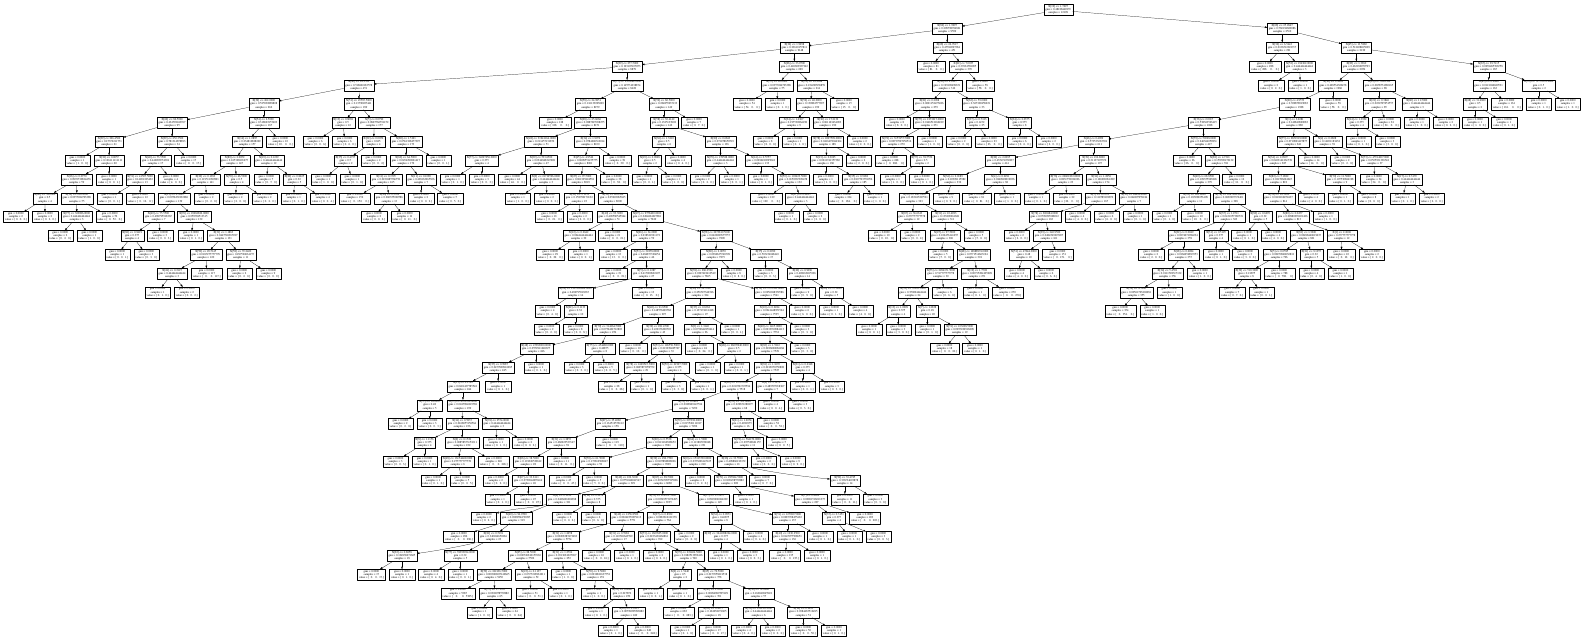
\includegraphics[width=0.6\textwidth]{img/ALL_ALL_1.png}
        \tiny{\caption[all-all-1]{\textbf{ALL Set Decision Tree}}}

        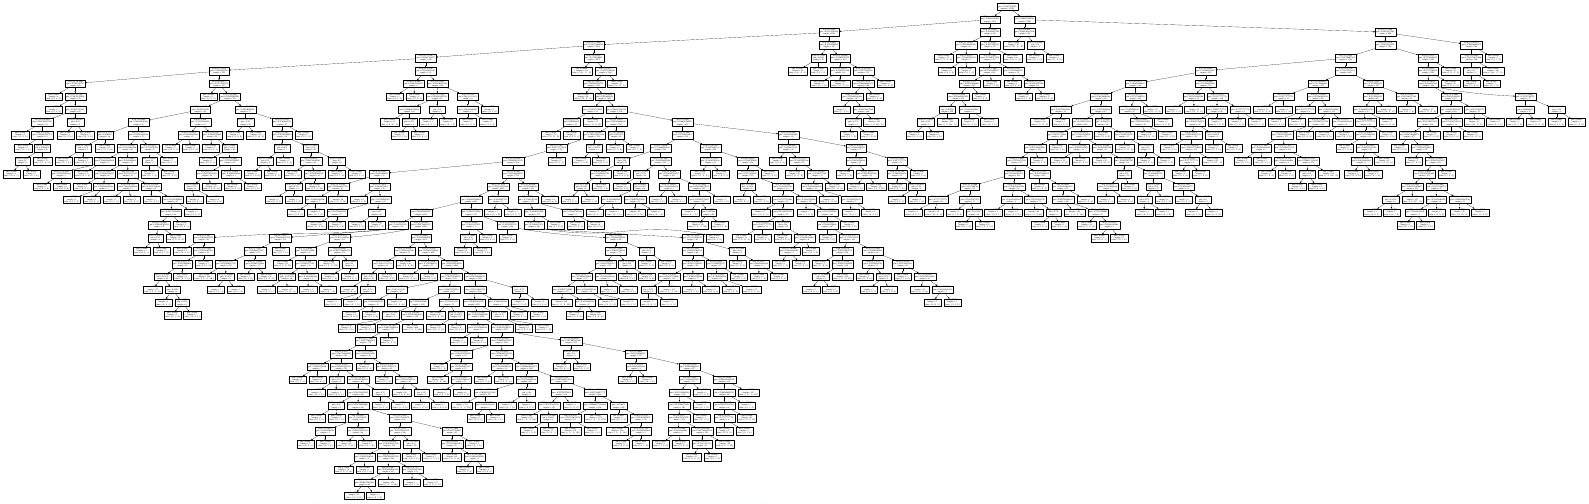
\includegraphics[width=0.6\textwidth]{img/ALL_AQC_1.png}
        \tiny{\caption[all-aqc-1]{\textbf{AQC Set Decision Tree}}}

        \tiny{https://github.com/SamStudio8/frontier/tree/master/results/front/}
    \end{figure}
\end{frame}

\begin{frame}[t]
    \frametitle{Overfitting}
    \begin{figure}[htbp!]
        \centering
        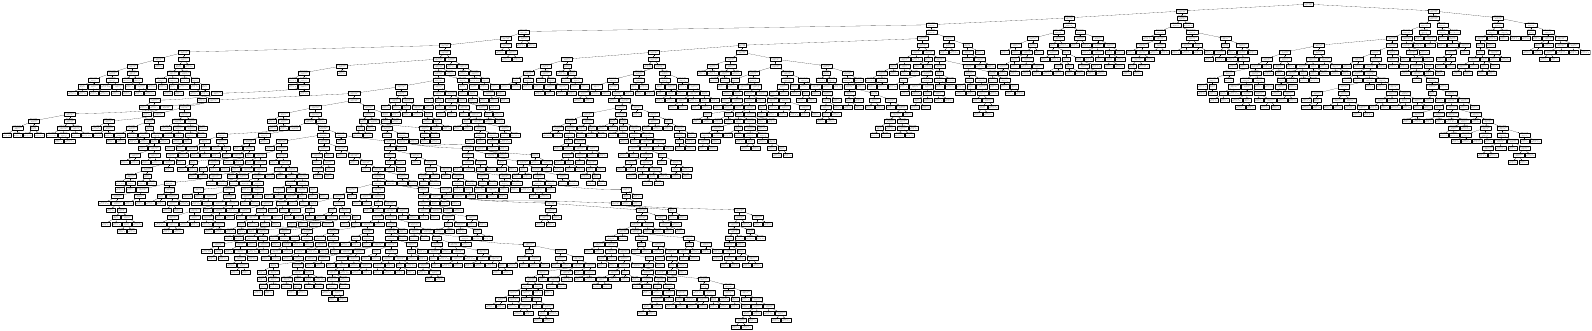
\includegraphics[width=\textheight,height=3cm]{img/ALL_BASELINE_1.png}
        \tiny{\caption[all-baseline-1]{\textbf{BASELINE Set Decision Tree}}}

        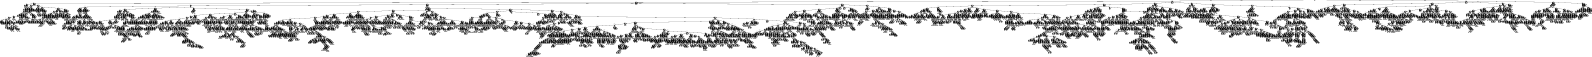
\includegraphics[width=\textheight,height=1.5cm]{img/ALL_ERROR_1.png}
        \tiny{\caption[all-error-1]{\textbf{ERROR Set Decision Tree}}}

        \tiny{https://github.com/SamStudio8/frontier/tree/master/results/front/}
    \end{figure}
\end{frame}

\begin{frame}[t]
\frametitle{Augmenting Warning Handling}
    \begin{table}
        \centering
        \tiny
        \begin{tabular}{l l | c  c  c  c  r}
            PSet & DSet          & \# & CV $±$ SD & SCV $±$ SD & Depth & Most Important Feature\\
            \hline
            ALL & IGNWARN    & 86 & 96 $±$ 3 & 99 $±$ 0 & 22 & error-rate (43\%)\\
            ALL & WARNPASS   & 86 & 95 $±$ 3 & 99 $±$ 0 & 33 & quality-dropoff-rev-mean-runmed\\
                                                        &&&&&&-decline-low-value (32\%)\\
            AQC & IGNWARN    & 27 & 94 $±$ 4 & 98 $±$ 1 & 26 & error-rate (44\%)\\
            AQC & WARNPASS   & 27 & 92 $±$ 4 & 98 $±$ 1 & 33 & quality-dropoff-rev-mean-runmed\\
                                                        &&&&&&-decline-low-value (33\%)\\
        \end{tabular}

        \caption[all-pset-cv]{\tiny{\textbf{Parameter Set Cross Validation Scores using
            Alternative Warning Handling}:
            Results of classifying testing data.
            Columns left to right; parameter set name, data set name, number of parameters
            included, average cross-validation score (max 100) $±$ std. deviation,
            average stratified cross-validation score (max 100) $±$ std. deviation,
            average depth of the generated tree and the most important parameter by
            Gini importance (max 100). Tree depth and parameter importance was
            estimated on experiments using the stratified data. \textit{N.B.}
            \textbf{IGNWARN} and \textbf{WARNPASS} data sets perform classifications on
    two classes (pass and fail) rather than three.}}
    \end{table}
    \begin{itemize}
        \item \textbf{IGNWARN} discards, \textbf{WARNPASS} recodes as pass
        \item Very high validation, appears noise has been significant reduced
            when compared to the previously tabulated results
        \item Average maximum depth reduced
    \end{itemize}
\end{frame}

\begin{frame}[t]
\frametitle{Backward Elimination}
    \begin{columns}[c]
        \column{5cm}
            \begin{table}[H]
                \centering
                \tiny
                \begin{tabular}{l}
                    A-percent-mean-below-baseline                     \\
                    duplicate-mapped-ratio                            \\
                    fwd-percent-insertions-above-baseline             \\
                    insert-size-average                               \\
                    max-max-baseline-deviation                        \\
                    quality-dropoff-fwd-mean-runmed-decline-low-value \\
                    quality-dropoff-rev-mean-runmed-decline-low-value \\
                    rev-percent-insertions-above-baseline             \\
                    rev-percent-insertions-below-baseline             \\
                \end{tabular}

                \tiny{\caption[top9-params]{\tiny{\textbf{TOP9 Parameter Set}: Features selected by a
                    backward elimination experiment providing all observations to an
                    iterative decision tree classifier and removing the least important
                    feature until cross-validation fell below a threshold.
        }}}
            \end{table}
        \column{7cm}
            \begin{itemize}
                \item Borrowed a method from statistical model design
                \item Repeatedly refitted trees after removing the least important feature
                    until cross-validation fell below some percentage of the running average
                \item Would be very interesting to repeat this process for various
                    augmentations of the warnings class handling
            \end{itemize}
    \end{columns}
\end{frame}

\begin{frame}[t]
\frametitle{TOP9 Experiment Results}
    \begin{table}
        \centering
        \tiny
        \begin{tabular}{l l | c  c  c  c  r}
            PSet & DSet          & \# & CV $±$ SD & SCV $±$ SD & Depth & Most Important Feature\\
            \hline
            RTOP9 & ALL         & 9  & 87 $±$ 6  & 95 $±$ 1 & 32 & max-max-baseline-deviation (32\%)\\
            RTOP9 & IGNWARN     & 9  & 98 $±$ 1  & 99 $±$ 0 & 20 & rev-pct-insertions-above-baseline (38\%)\\
            RTOP9 & WARNPASS    & 9 & 95 $±$ 3 & 99 $±$ 1 & 24 &
                                                        quality-dropoff-rev-mean-runmed\\
                                                        &&&&&&-decline-low-value (34\%)\\
        \end{tabular}

        \caption[be-pset-cv]{\tiny{\textbf{Backward Elimination Parameter Set Cross Validation Scores}:
            Results of classifying testing data.
            Columns left to right; parameter set name, data set name, number of parameters
            included, average cross-validation score (max 100) $±$ std. deviation,
            average stratified cross-validation score (max 100) $±$ std. deviation,
            average depth of the generated tree and the most important parameter by
            Gini importance (max 100). Tree depth and parameter importance was
            estimated on experiments using the stratified data. \textit{N.B.}
            \textbf{IGNWARN} and \textbf{WARNPASS} data sets perform classifications on
            two classes (pass and fail) rather than three.}}
    \end{table}
    \begin{itemize}
        \item Impressive validation results considering only 9 parameters
        \item Average maximum tree depth upper bound briefly overlaps the lower bound
            of the results found from the naive parameter sets
        \item Clearly we can gain accuracy on class prediction without the need for
            including every parameter in the model, \textbf{TOP9} is even smaller than the
            \textbf{AQC} set!
    \end{itemize}
\end{frame}

\begin{frame}[t]
    \frametitle{TOP9 Decision Tree with All Data}
    \begin{figure}[htbp!]
        \centering
        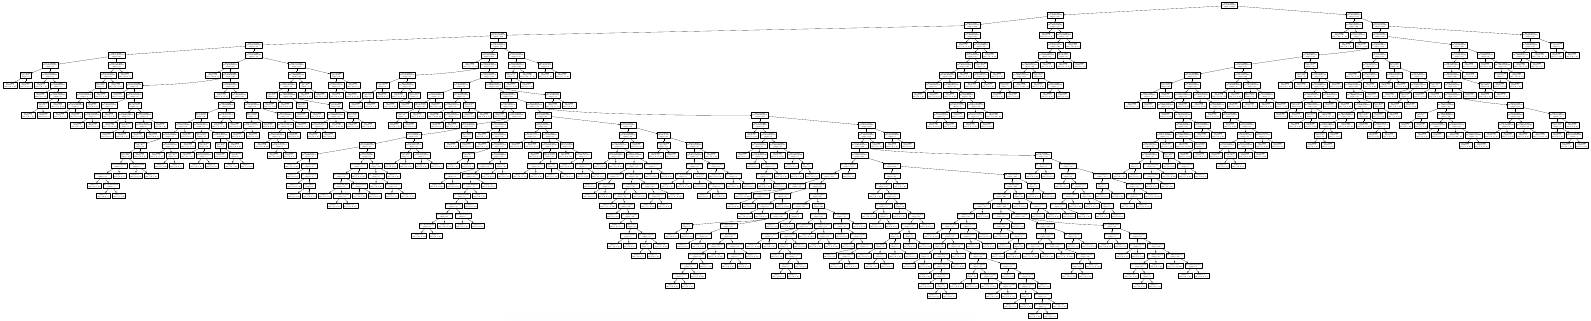
\includegraphics[width=1\textwidth]{img/TOP9_ALL_1.png}
        \tiny{\caption[top9-all-1]{\textbf{TOP9 Set Decision Tree with ALL Data}}}

        \tiny{https://github.com/SamStudio8/frontier/tree/master/results/front/}
    \end{figure}
    \begin{itemize}
        \item More complex structure and larger size than previous figures that
            include all parameters
        \item Further experimentation with the stopping criteria of the backward
            elimination process should be considered
    \end{itemize}
\end{frame}

\begin{frame}[t]
    \frametitle{TOP9 Decision Trees with Warning Augmentations}

    \begin{columns}[c]
    \column{6cm}
        \begin{figure}[htbp!]
            \centering
            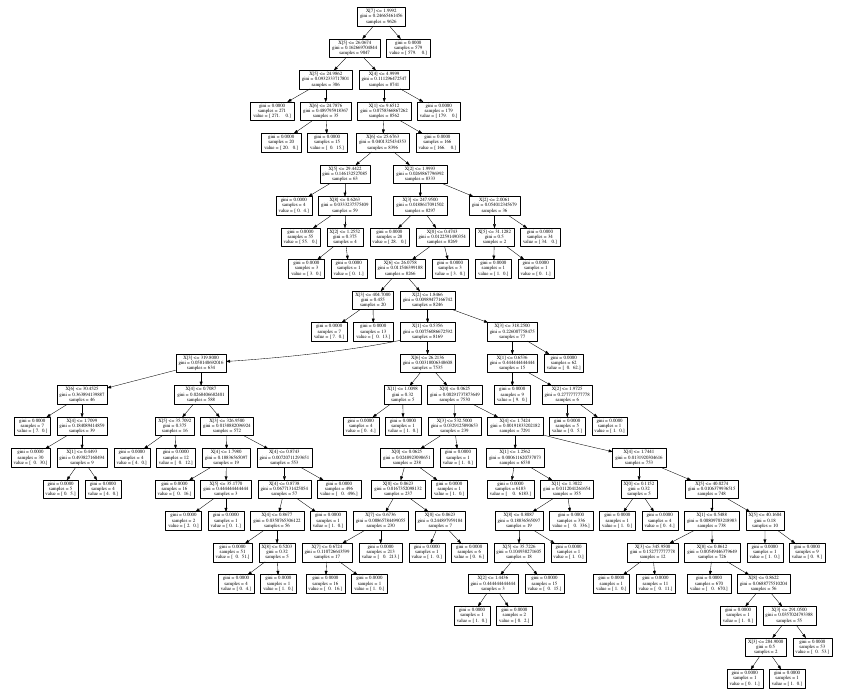
\includegraphics[width=1\textwidth]{img/TOP9_IGNWARN_1.png}
            \tiny{\caption{\textbf{TOP9 Set Decision Tree with IGNWARN Data}}}
        \end{figure}
    \column{6cm}
        \begin{figure}[htbp!]
            \centering
            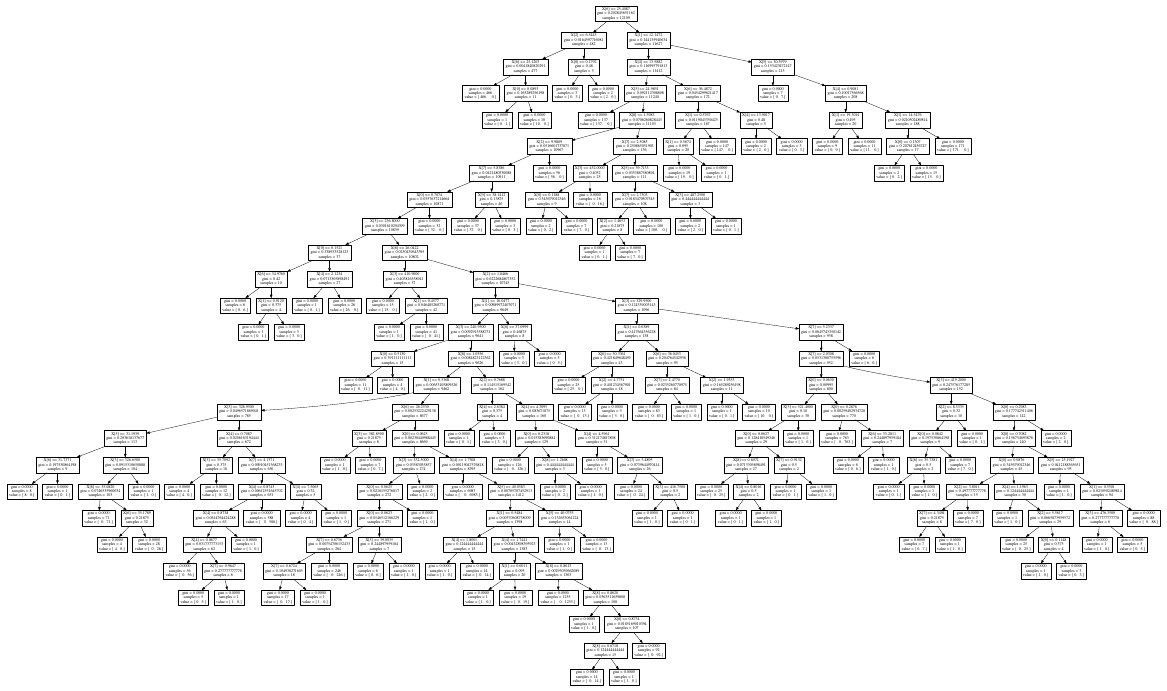
\includegraphics[width=1\textwidth]{img/TOP9_WARNPASS_1.png}
            \tiny{\caption{\textbf{TOP9 Set Decision Tree with WARNPASS Data}}}
        \end{figure}
    \end{columns}
    \centering
    \tiny{https://github.com/SamStudio8/frontier/tree/master/results/front/}
\end{frame}

\begin{frame}[t]
    \frametitle{TOP9 Example Decision Path}

    \begin{columns}[c]
    \column{6cm}
        \begin{figure}[htbp!]
            \centering
            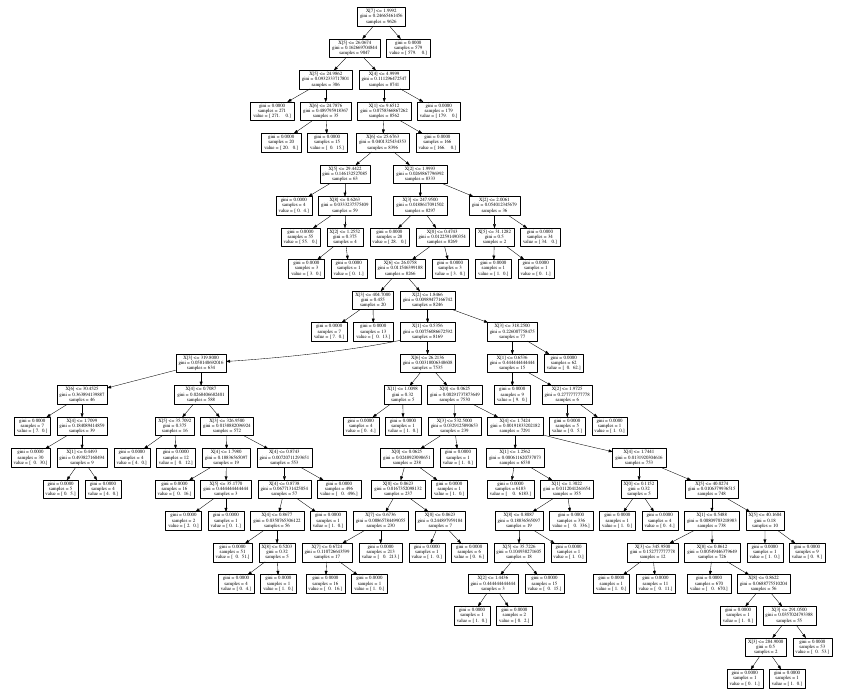
\includegraphics[width=1\textwidth]{img/TOP9_IGNWARN_1.png}
            \tiny{\caption{\textbf{TOP9 Set Decision Tree with IGNWARN Data}}}
        \end{figure}
    \column{6cm}
        \begin{itemize}
            \item Paths still exhibit some element of arbitrariness
            \item Need to further investigate criteria for backward elimination
            \item Surprised that the set is much smaller than \textbf{AQC}
            \item Sensible to investigate some form of pruning to further remove
                smaller leaves
        \end{itemize}
    \end{columns}
    \centering
    \tiny{https://github.com/SamStudio8/frontier/tree/master/results/front/}
\end{frame}

%%%%%%%%%%%%%%%%%%%%%%%%%%%%%%%%%%%%%%%%%%%%%%%%%%%%%%%%%%%%%%%%%%%%%%%%% IntroP2
\section{Part II}
\subsection{Reminder}

\begin{frame}[t]
\frametitle{Aims}
    \begin{beamerboxesrounded}[shadow=true]{}
        \begin{center}
            Identify lanelet properties that affect downstream variant calling
        \end{center}
    \end{beamerboxesrounded}
    \uncover<1>{
        \begin{itemize}
            \item For better QC we need an idea of "good" and "bad"
            \item How does quality affect analyses performed after sequencing?
        \end{itemize}
    }
    \uncover<2>{
        \vskip 0.5cm
        \begin{beamerboxesrounded}[shadow=true]{}
            \begin{center}
                Goals
            \end{center}
        \end{beamerboxesrounded}
        \begin{itemize}
            \item Will leaving out a sample during variant calling affect the result?
            \item Select a "representative" region of the human genome for analysis
            \item Compare calls on whole genome samples to "SNP chips"
            \item Determine what is actually "good" and "bad" for QC
        \end{itemize}
    }
\end{frame}

%%%%%%%%%%%%%%%%%%%%%%%%%%%%%%%%%%%%%%%%%%%%%%%%%%%%%%%%%%%%%%%%%%%%%%% P2: Gold
\section{Goldilocks}
\subsection{Goldilocks}

\begin{frame}[t]
\frametitle{Searching for Goldilocks}
    \begin{beamerboxesrounded}[shadow=true]{}
        \begin{center}
            Introducing \textbf{Goldilocks}
        \end{center}
    \end{beamerboxesrounded}
    \begin{itemize}
        \item Need to locate an appropriate region for the pipeline to minimise
            computational time and resources
        \item Representative region -- not too many or too few variants
        \item Need to handle variant data from two different types of study
        \item A Python module capable of parsing files containing chromosome-position
            pairs and conducting a variant census
        \item Filter and ranks censused regions of a genome based on the number of
            variants contained
        \item Presents an API to allow users to call any desired part of the module
            from other programs and scripts
    \end{itemize}
\end{frame}


\begin{frame}[t]
\frametitle{Top 25 1Mnt Goldilocks Regions}
    \begin{columns}[c]
    \column{7.5cm}
        \begin{table}[H]
            \tiny
            \centering
            \begin{tabular}{l | c  c  c  r  r}
                i & GWAS & iCHIP & Chr & Start & End \\
                \hline
                0234&297&470&1& 117,000,001 &  118,000,000\\
                1074*&294&1540&3&  46,000,001 &   47,000,000\\
                5222&294&336&21&  16,500,001 &   17,500,000\\
                3125&298&310&10&  60,000,001 &   61,000,000\\
                0880&293&344&2& 191,500,001 &  192,500,000\\
                3560&299&772&12&   9,000,001 &   10,000,000\\
                4407&299&512&15&  78,500,001 &   79,500,000\\
                1036&292&300&3&  27,000,001 &   28,000,000\\
                2734&300&515&9&   5,000,001&    6,00,0000\\
                3426&300&486&11&  76,000,001 &   77,000,000\\
                0015&291&1029&1&   7,500,001 &    8,500,000\\
                0365&301&487&1& 182,500,001 &  183,500,000\\
                3415&301&419&11&  70,500,001 &   71,500,000\\
                1581&290&802&4& 102,500,001 &  103,500,000\\
                3554&290&403&12&   6,000,001 &    7,000,000\\
                3184&302&449&10&  89,500,001 &   90,500,000\\
                1580&289&603&4& 102,000,001 &  103,000,000\\
                1948&288&1297&5&  96,000,001 &   97,000,000\\
                2215&288&622&7&  49,500,001 &   50,500,000\\
                0414&288&346&1& 207,000,001&  208,000,000\\
                2055&304&1377&5& 149,500,001 &  150,500,000\\
                0384&287&827&1& 192,000,001 &  193,000,000\\
                0959&306&406&2& 231,000,001 &  232,000,000\\
                4214&286&393&14&  88,500,001 &   89,500,000\\
                0320&307&620&1& 160,000,001 &  161,000,000\\
            \end{tabular}
        \end{table}
    \column{5cm}
        \begin{itemize}
            \item Filtered by median GWAS (297), ranked by maximum iCHIP
            \item Initially required over an hour to process the human genome,
                now completes the task in less than 20 seconds
            \item Avoided chromosome 6 due to presence of HLA system
            \item Suitable candidate 1074(*) located on chromosome 3
        \end{itemize}
    \end{columns}
\end{frame}


\begin{frame}[t]
    \frametitle{GWAS vs. iCHIP Variant Densities}
    \centering
    \resizebox{0.88\textwidth}{!}{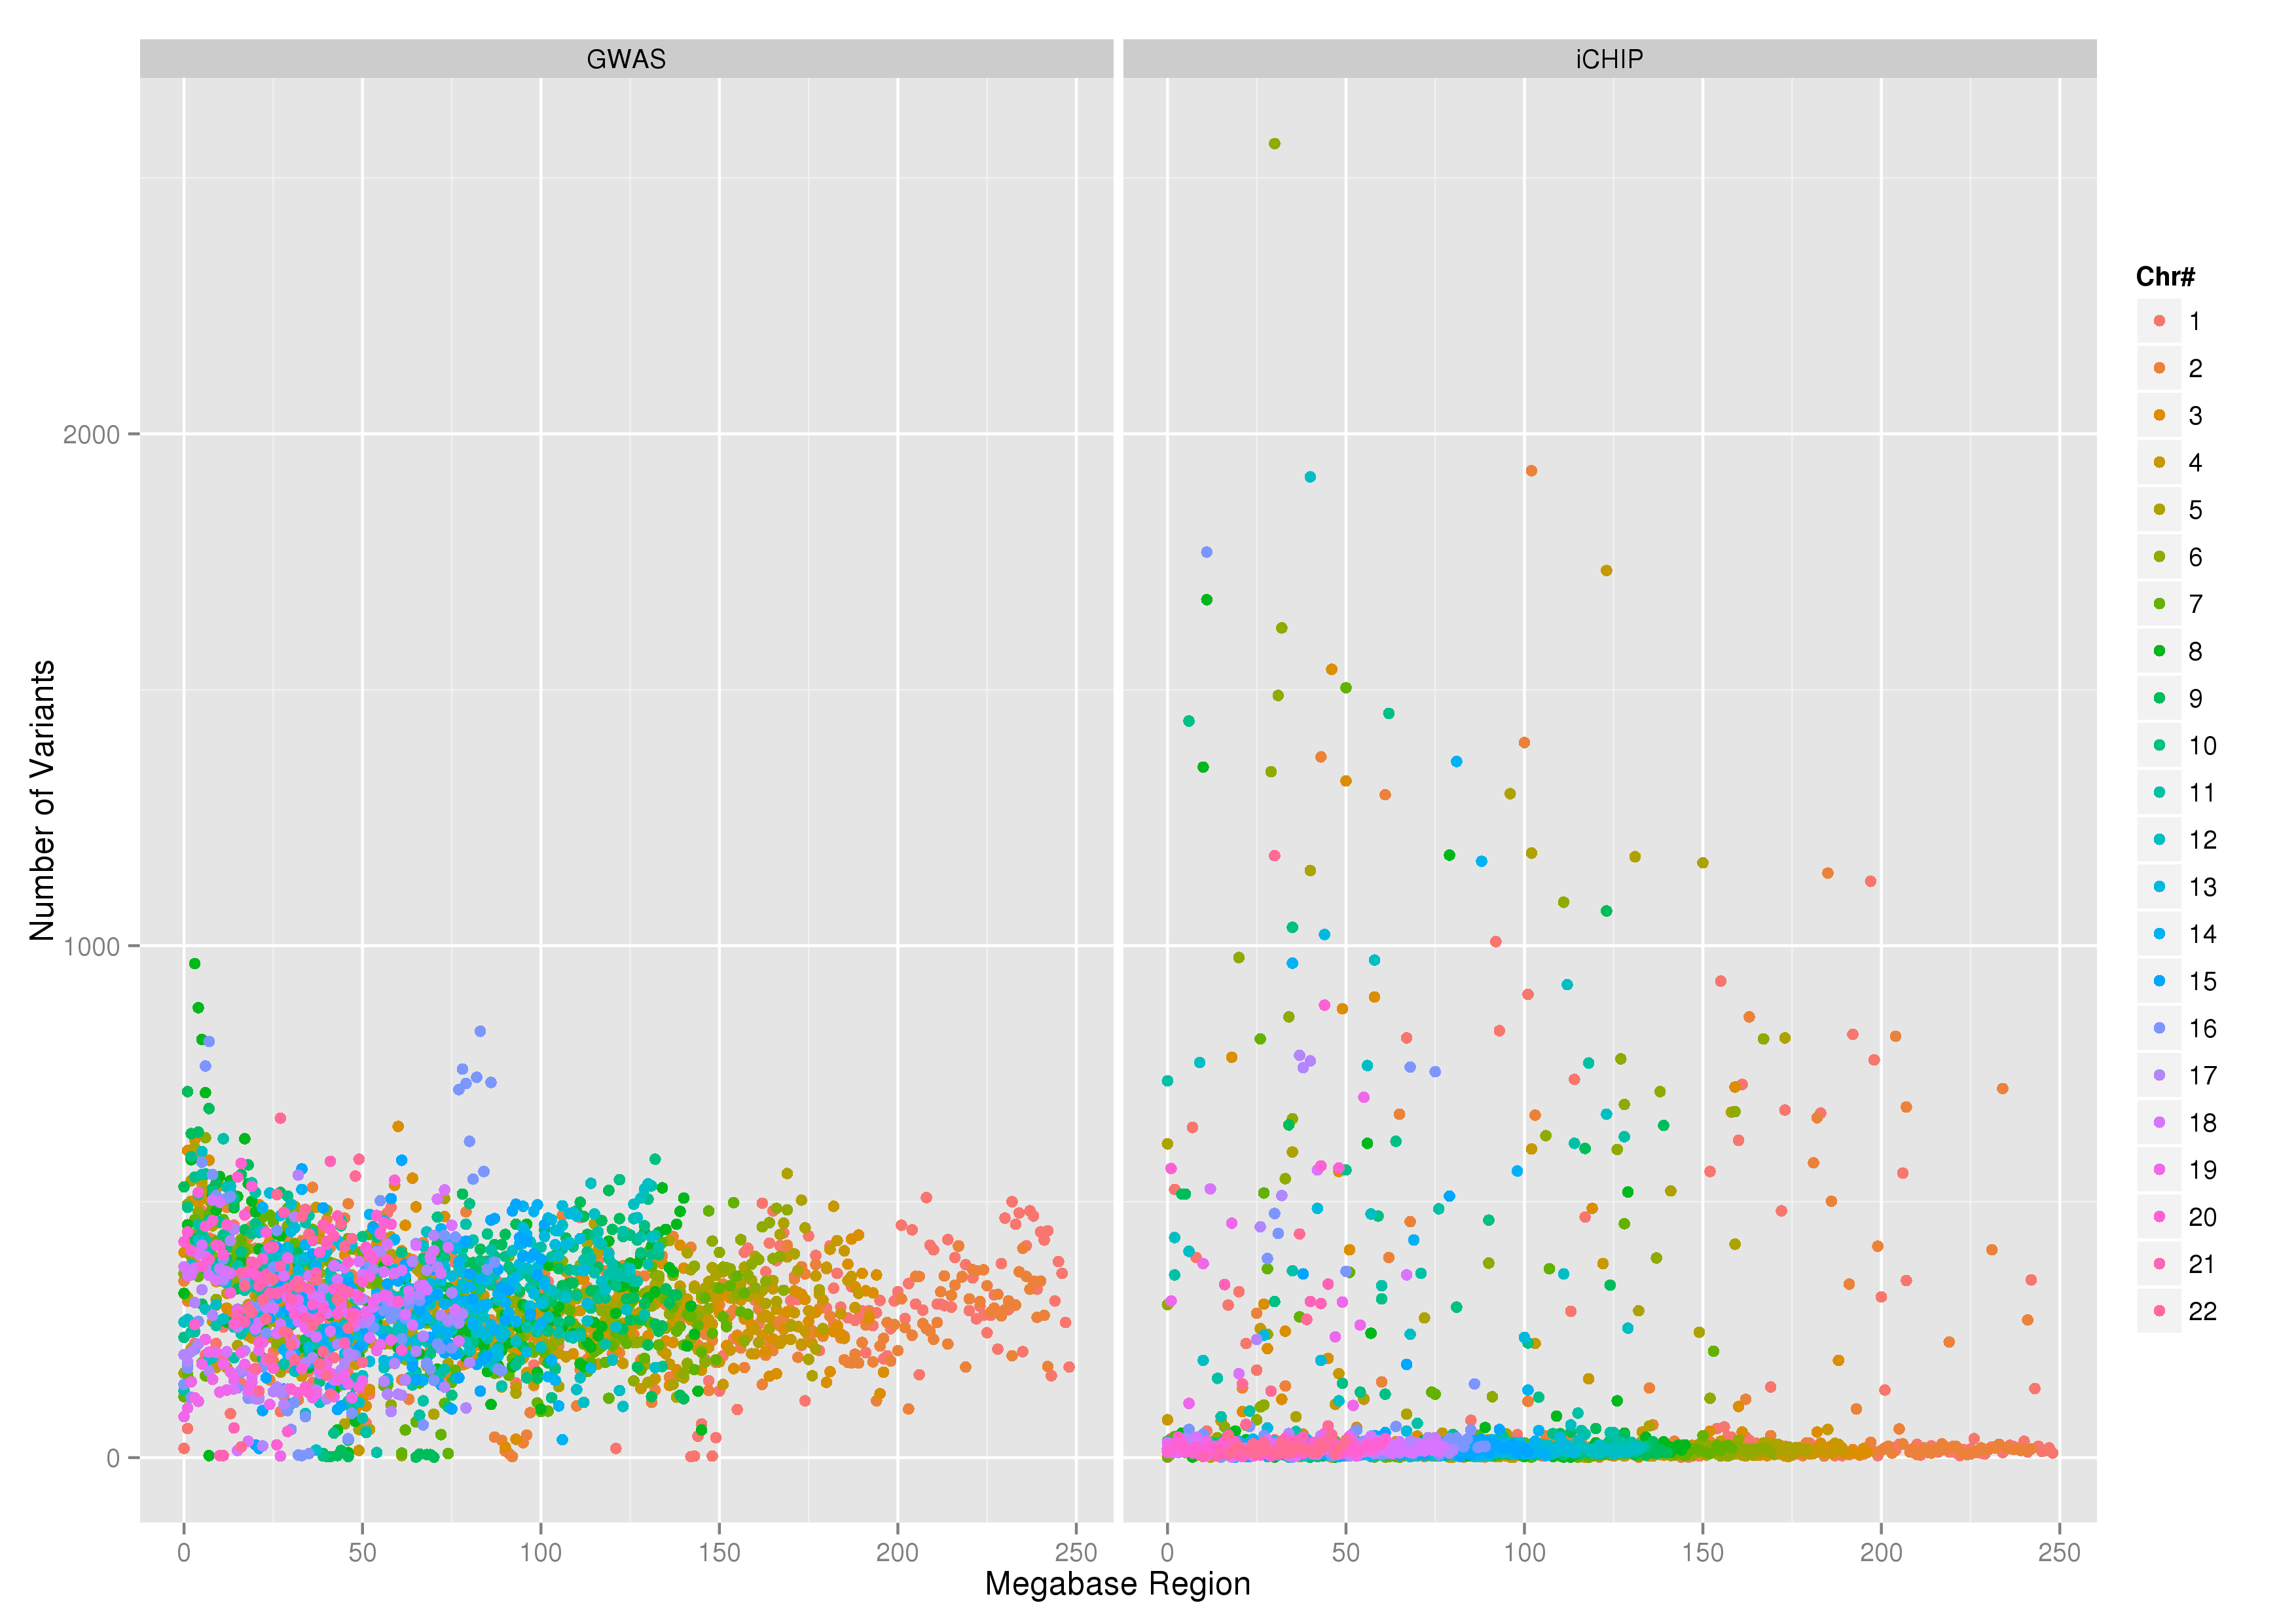
\includegraphics{img/megabase_plot.png}}
\end{frame}
\begin{frame}[t]
    \frametitle{GWAS vs. iCHIP Variant Densities}
    \centering
    \resizebox{0.88\textwidth}{!}{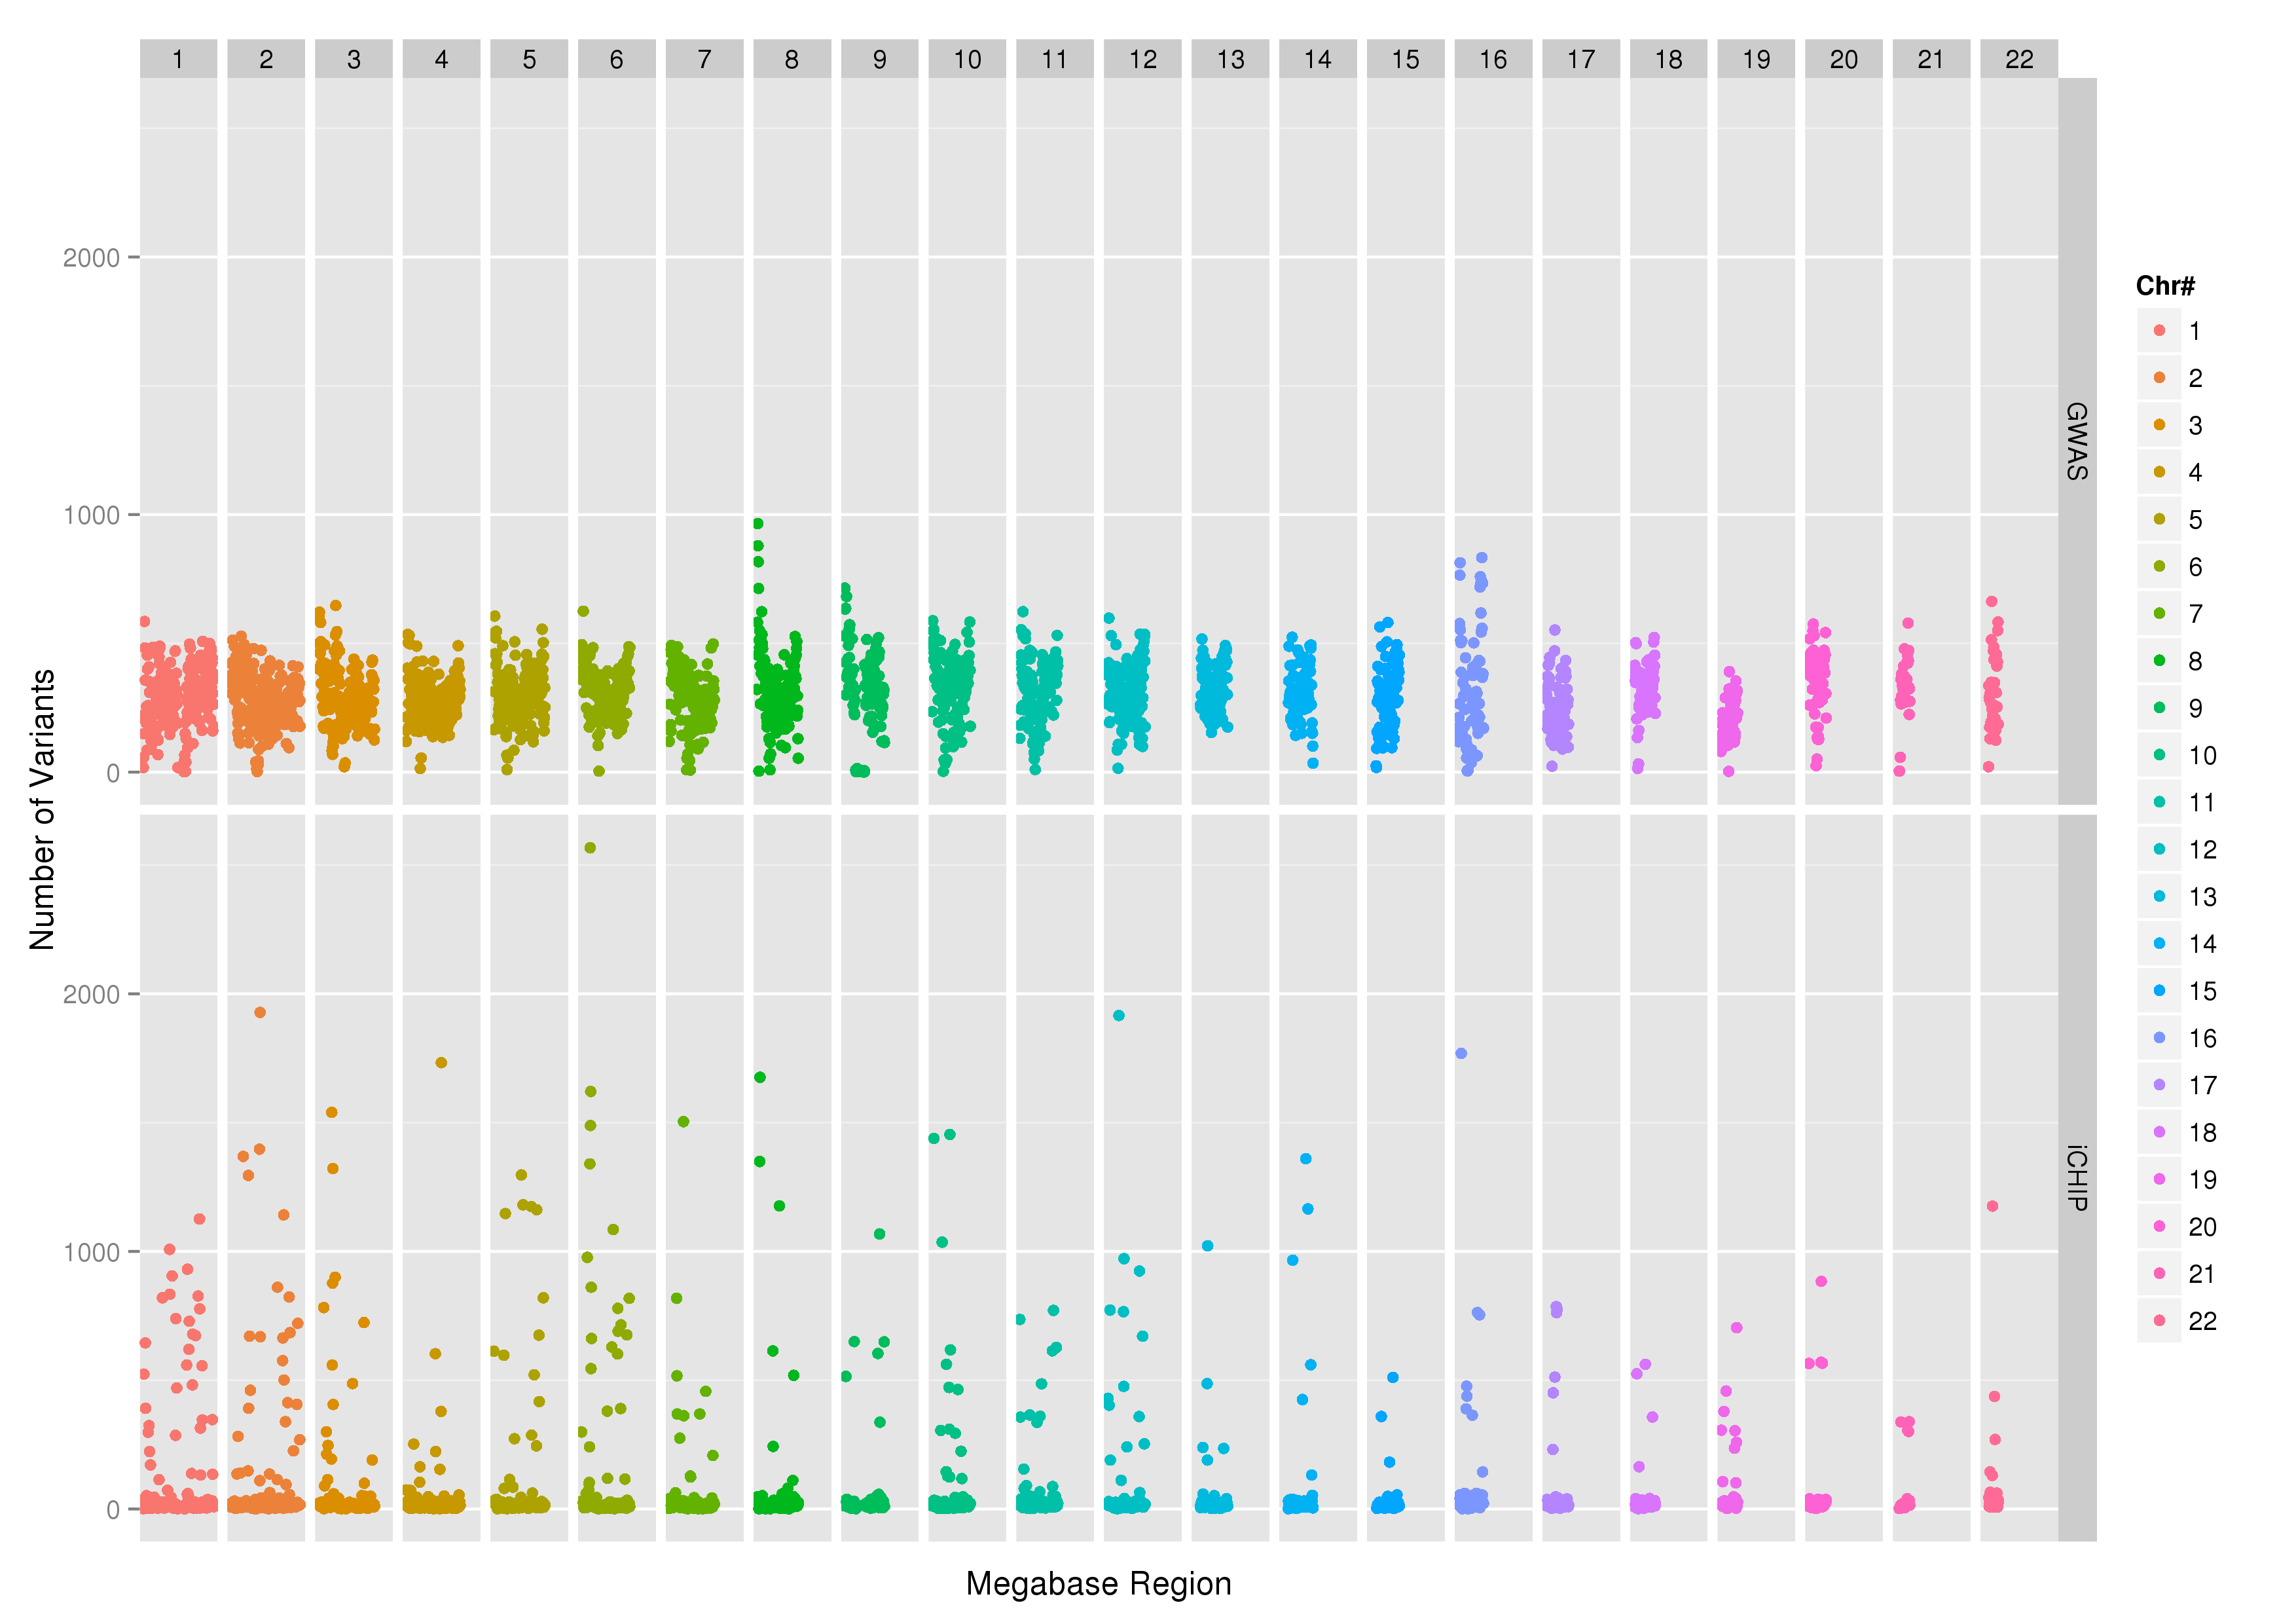
\includegraphics{img/megabase_plot_split.png}}
\end{frame}


%%%%%%%%%%%%%%%%%%%%%%%%%%%%%%%%%%%%%%%%%%%%%%%%%%%%%%%%%%%%%%%%%%%%%% P2: Pipe
\section{Pipeline}
\subsection{Pipeline}

\begin{frame}[t]
\frametitle{Pipeline Components}
    \begin{itemize}
        \uncover<1>{
            \item \textbf{Extraction} \hfill\\
                Extract the Goldilocks region for all \textbf{GWAS} study lanelets
        }
        \uncover<2>{
            \item \textbf{Indexing} \hfill\\
                Create indexes for the extracted Goldilocks regions
        }
        \uncover<3>{
            \item \textbf{Merge} \hfill\\
                Merge the data from each extracted region into one file
        }
        \uncover<4>{
            \item \textbf{Pileup} \hfill\\
                Calculate genotype likelihoods based on the reads seen across all the
                extracted regions
        }
        \uncover<5>{
            \item \textbf{Call} \hfill\\
                Use the genotype likelihood scores to call the variants for
                each position of interest in each of the Goldilocks regions
        }
        \uncover<6>{
            \item \textbf{Compare} \hfill\\
                For each pair of \textbf{GWAS} and \textbf{iCHIP} samples, measure the
                concordance of called variants
        }
    \end{itemize}
\end{frame}


\begin{frame}[t]
\frametitle{Pipeline Difficulties: Pileup and Calling}
    \uncover<1>{
        \begin{beamerboxesrounded}[shadow=true]{}
            \begin{center}
                Scaling \textbf{samtools mpileup}
            \end{center}
        \end{beamerboxesrounded}
        \begin{itemize}
            \item Executing a pileup is a performance intensive task
            \item Initial test runs required 6.5 hours of CPU time with 1GB RAM
            \item Significant overhead with thousands of sample files, couldn't have
                performed this step multiple times without merging
        \end{itemize}
    }

    \uncover<2>{
        \begin{beamerboxesrounded}[shadow=true]{}
            \begin{center}
                Compatibility with \textbf{bcftools call}
            \end{center}
        \end{beamerboxesrounded}
        \begin{itemize}
            \item Produced only standard header information and no data as the pileup
                task had not included an appropriate reference sequence
            \item Using \texttt{--M} flag for \textit{masked reference} caused software
                to segmentation fault instead
            \item Needed to rebuild all libraries due to compatibility trouble
        \end{itemize}
    }
\end{frame}

\begin{frame}[t]
\frametitle{Pipeline Difficulties: Merging}
    \uncover<1>{
        \begin{beamerboxesrounded}[shadow=true]{}
            \begin{center}
                Documentation for \textbf{samtools merge}
            \end{center}
        \end{beamerboxesrounded}
        \begin{itemize}
            \item Filed pull request to document feature allowing a file of filenames
                to be provided as an input instead of listing on command line
        \end{itemize}
    }

    \uncover<2>{
        \begin{beamerboxesrounded}[shadow=true]{}
            \begin{center}
                Memory Leaks in \textbf{samtools merge}
            \end{center}
        \end{beamerboxesrounded}
        \begin{itemize}
            \item Merge jobs repeatedly killed for excessive memory use by LSF
            \item Discovered several memory leaks whose severity increased proportionally
                to the number of input files -- fixed by author
            \item During testing I tracked down and patched several memory leaks in both 
                the \textbf{merge} and \textbf{split} testing harnesses using \textbf{valgrind}
            \item Merge jobs then repeatedly killed for exceeding time limits
        \end{itemize}
    }
\end{frame}

\begin{frame}[t]
\frametitle{Pipeline Difficulties: Merging}
    \begin{beamerboxesrounded}[shadow=true]{}
        \begin{center}
            Time Sinks in \textbf{samtools merge}
        \end{center}
    \end{beamerboxesrounded}
    \begin{itemize}
        \item Experimented with \textbf{callgrind} to search for heavily used
            functions or particularly costly calls
        \item Found many expensive calls to \textbf{zlib} -- an open source
            compression library -- when compressing the output
        \item Turned out to be proportionally insignificant, using uncompressed output
            still led to long execution times
        \item Tried \textbf{gprof} to look at actual execution time rather than
            CPU instruction count, found 50\% of execution time was spent searching
            for tags in data structures
        \item Number of files causes non-linear increase in time,
            now currently believe implementation of header parsing is very inefficient
            and just cannot scale in current form
    \end{itemize}
\end{frame}


%%%%%%%%%%%%%%%%%%%%%%%%%%%%%%%%%%%%%%%%%%%%%%%%%%%%%%%%%%%%%%%%%%%% Conclusion
\section{Conclusion}
\subsection{Conclusion}

\begin{frame}[t]
\frametitle{Conclusion}
    \begin{beamerboxesrounded}[shadow=true]{}
        \begin{center}
            Critical Evaluation
        \end{center}
    \end{beamerboxesrounded}
    \begin{itemize}
        \item \textbf{Frontier} greatly assisted the analysis conducted in Part I
        \item Happy with choice of Python and \textbf{scikit-learn}, project benefits
            from mutual use of \textbf{NumPy} containers and functions
        \item Many interesting lines of questioning introduced in Part I results
        \item Demonstrated in brief that decision trees generated exhibit similar
            behaviour to the currently existing \textbf{auto\_qc} system
        \item Encouraging progress in both Part I and II but ultimately cut short
            due to unexpected difficulties with the pipeline components
    \end{itemize}
\end{frame}

\begin{frame}[t]
\frametitle{Conclusion}
    \begin{beamerboxesrounded}[shadow=true]{}
        \begin{center}
            In summary this project...
        \end{center}
    \end{beamerboxesrounded}
    \begin{itemize}
        \item Introduced \textbf{Frontier}, a Python package providing users with
            interfaces for reading, storage and retrieval of large machine learning
            data sets
        \item Used \textbf{Frontier} and \textbf{scikit-learn} to conduct preliminary
            analysis as to whether behaviour of the current QC system could be recovered
            via machine learning
        \item Identified parameters (\textbf{TOP9}) that contribute to accurate
            classification and showed ignoring warnings reduces noise
        \item Created \textbf{Goldilocks} for locating an appropriate genomic
            region for use in Part II analysis
        \item Outlined a pipeline for processing thousands of samples
        \item Produced contributions to widely used bioinformatics tools
    \end{itemize}
\end{frame}

\begin{frame}[t]
    \frametitle{Conclusion}
    \begin{beamerboxesrounded}[shadow=true]{}
        \begin{center}
            Future Plans
        \end{center}
    \end{beamerboxesrounded}
    \begin{itemize}
        \item Complete the assembly of the analysis pipeline (most likely requiring
            substantial additions to \textbf{samtools merge})
        \item Use concordance results from Part II to inform new lines of inquiry
            where Part I left off
        \item Continue development of \textbf{Frontier} and submit to \textbf{PyPi}
        \item Explore use of other machine learning algorithms and frameworks and
            their application to the task of quality control classification
        \item Investigate post-pruning algorithms and ensemble methods as decision
            trees cannot promise optimality
    \end{itemize}
\end{frame}

\begin{frame}[t]
    \frametitle{Conclusion}
    \vskip 2.5cm
    \begin{beamerboxesrounded}[shadow=true]{}
        \begin{center}
            Questions?
        \end{center}
    \end{beamerboxesrounded}
\end{frame}

\end{document}

